% --------------------------------------------------------------------------
% Template for ICAD-2021 paper; to be used with:
%          icad2021.sty  - ICAD 2021 LaTeX style file, and
%          IEEEbtran.bst - IEEE bibliography style file.
%
% --------------------------------------------------------------------------
\UseRawInputEncoding
\documentclass[a4paper,10pt,oneside]{article}
\usepackage{icad2021,amsmath,epsfig,times,url,hyperref}
\usepackage[utf8]{inputenc}
\usepackage{listings}
\usepackage{xcolor}

%New colors defined below
\definecolor{codegreen}{rgb}{0,0.6,0}
\definecolor{codegray}{rgb}{0.15,0.15,0.15}
\definecolor{codepurple}{rgb}{0.58,0,0.82}
\definecolor{backcolour}{rgb}{0.95,0.95,0.92}
% Example definitions.
% --------------------
\def\defeqn{\stackrel{\triangle}{=}}
\newcommand{\symvec}[1]{{\mbox{\boldmath $#1$}}}
\newcommand{\symmat}[1]{{\mbox{\boldmath $#1$}}}

% Title.
% --------------------
\title{DreamSound: Deep Activation Layer Sonification}

% *** IMPORTANT ***
% *** PLEASE LEAVE AUTHOR INFORMATION BLANK UNTIL FINAL CAMERA-READY SUBMISSION *** 

% IF ONE AUTHOR
%\name{Jyri Huopaniemi} 
%\address{Nokia Research Center \\ 
%Speech and Audio Systems Laboratory \\ 
%P.O.Box 407, FIN-00045 Nokia Group, Finland \\ 
%{\tt jyri.huopaniemi@nokia.com}} 
%

% IF TWO AUTHORS
\twoauthors{Federico Camara Halac} {Ohio State University\\ 1813 North High Street\\ Columbus, Ohio  \\ {\tt camarahalac.1@osu.edu}}
{Matias Delgadino} {Oxford University \\ Woodstock Road \\ Oxford, OX2 6GG  \\ {\tt matias.delgadino@maths.ox.ac.uk}}

\begin{document}
\ninept
\maketitle

\begin{sloppy}

\begin{abstract}
\end{abstract}

\section{Introduction}
\label{sec:intro}
Deep Learning (DL) in audio signal processing \cite{2019Purwins} has received much attention in the last four years \cite{choi2017tutorial, herremans2017proceedings}, and it is a growing field.\footnote{See, e.g., the Aalto courses on Deep Learning with Audio: \url{https://github.com/SopiMlab/DeepLearningWithAudio}} 
The Music Information Retrieval (MIR) community incorporated DL via large-scale audio datasets that came as early as 2015 and 2017 \cite{2015piczak,2017audioset,engel2017neural}, namely in relation to classification\footnote{
Despite the usefulness of DL in raw audio, e.g. it reduces the gap between symbolic and audio classification \cite{sergio_oramas_2017_1417427}, not all MIR problems benefit from it \cite{harsh_verma_2019_3527866}.
}, fundamental frequency estimation \cite{rachel_m_bittner_2017_1417937,kim2018}, and less so for synthesis. Particularly in the latter case, the use of Generative Adversarial Nets proved successful \cite{Bollepalli_2017, oord2017parallel, 2017Kaneko, pascual2017segan, 2019waveglow, tian2020tfgan, Liu_2020}.\footnote{
Some examples within the last four years are: 
genre classification \cite{sergio_oramas_2017_1417427}, 
singing voice separation \cite{andreas_jansson_2017_1414934}, 
instrument activity detection \cite{siddharth_gururani_2018_1492479}, 
instrument classification \cite{juan_s_gomez_2018_1492481}, 
downbeat tracking \cite{magdalena_fuentes_2018_1492355}, 
optical music recognition \cite{lukas_tuggener_2018_1492401}, 
mood detection \cite{remi_delbouys_2018_1492427}, 
tempo estimation \cite{hadrien_foroughmand_2019_3527890},
key classification \cite{fu_zih_sing_2019_3527960}, 
beat-tracking \cite{akira_maezawa_2017_1415520,magdalena_fuentes_2019_3527792}, 
sequence classification \cite{sathwik_tejaswi_madhusudhan_2019_3527862}, 
music analogy \cite{ruihan_yang_2019_3527880}, 
drum transcription \cite{keunwoo_choi_2019_3527774}, 
mood classification \cite{filip_korzeniowski_2020_4245488}, 
source separation \cite{petermann2020deep}, 
unison singing \cite{pritish_chandna_2020_4245502},

% voice separation in symbolic music \cite{reinier_de_valk_2018_1492403}, 

} 
Of the work at the intersection of DL and audio, a handful of examples relate to musical tasks. 
WaveNet was the first deep Convolutional Neural Network (CNN) for generating raw audio \cite{oord2016wavenet}. 
Other types of network followed, for example SampleRNN, with the use of Recurrent Neural Networks (RNN) \cite{mehri2017samplernn} and later \cite{kalchbrenner2018efficient}. 
An important advancement in the interpretation of Machine Listening models in \cite{saumitra_mishra_2018_1492527}, where they prove via feature inversion that temporal and harmonic structures are preserved in deep convolutional layers. 

The heavy computational requirements of these first architectures were later optimized with the goal being making faster architectures to achieve real-time synthesis, for example, with parallel computations \cite{oord2017parallel,yamamoto2020parallel,song2021improved}, and by using conditioning features \cite{lamtharn_hantrakul_2019_3527860}


Later, WaveGAN  \cite{Bollepalli_2017, donahue2018adversarial} and the multiple variants to GANs have appeared in the literature: 
conditional GAN \cite{2018Lee}, 
MelGAN \cite{NEURIPS2019_6804c9bc, jang2021universal}, 
WGANSing \cite{Chandna_2019}, 
TFGAN \cite{tian2020tfgan}, 
DRUMGAN \cite{javier_nistal_2020_4245504}, 
SyleMelGAN \cite{mustafa2021stylemelgan}.
These ground-breaking projects were all raw-audio based, and because of this, their architectures were aimed to generate short-length audio files. 
The authors worked on a past project, Kwgan, extending WaveGan to a conditional GAN geared to build large-scale audio databases for electroacoustic music material. In this case, raw audio is inputted for training and outputted for artistic or musically relevant contexts. 
A major breakthrough from \cite{oord2016wavenet} and \cite{mehri2017samplernn} comes with the WaveNET-like autoencoder in \cite{engel2017neural}, created as a new, data-driven synthesis technique for longer length audio files, extending GANs towards musical application. 
Several hybrid synthesizer models have been trained \cite{mccarthy2020hooligan}, and the first GAN synthesizer appeared \cite{engel2019gansynth}, trained on the NSynth dataset \cite{engel2017neural}, and the EnvGAN \cite{madhu2021envgan}, trained on the ESC dataset \cite{2015piczak} for environmental sound generation. 

% Magenta Studio: Augmenting Creativity with Deep Learning in Ableton Live
% rachel_manzelli_2018_1492375 symbolic conditioning 
%  symbolic gan : hao_wen_dong_2018_1492377 MUSEGAN: https://salu133445.github.io/musegan/papers
The literature reflects that one inspiration for the GAN application in sound came from the DCGAN\cite{radford2015unsupervised}, an architecture implemented to generate images based on adversarial training. 
The success of this application in images resonated well with the audio application of GANs. 

While other translations of deep architectures designed for image data to sound data have not given overwhelming results, particularly those involving spectrograms, what the success of GANs suggests is that using raw audio adds the temporal element needed for satisfactory sound results.\footnote{See here for an elaboration: \url{https://towardsdatascience.com/whats-wrong-with-spectrograms-and-cnns-for-audio-processing-311377d7ccd}} One example treats audio synthesis as a style-transfer problem, using back-propagation to optimize the sound to conform to filter from a pre-trained neural architecture \cite{verma2018neural}. However, the authors provide no audio examples besides the spectrogram display of their results. Of particular interest for our project, is thus a satisfactory translation of image to audio architectures. Particularly, the Deep Dream project, geared towards image generation using layer information within InceptionNet, a deep architecture previously built and trained for classification. The output of the Deep Dream, which can be understood as an image effect, is an image that is either modified or completely generated by the neural network itself, hence calling it \texit{dream}, raising further questions about the nature of networks and the otherness of AI.\footnote{The use of the word `dream' in the Deep Dream project comes from the metaphor that emerged from the resemblance of the Neural Network to the human brain.} In the present project, we present DreamSound\footnote{\url{https://github.com/fdch/dreamsound}}, an adaptation of the Deep Dream project into an audio-based musical context. DreamSound uses YAMNet\footnote{\url{https://tfhub.dev/google/yamnet/1}}, a novel sound classification deep convolutional network trained on the YouTube AudioSet. In section 1 we present our approach in relation to previous examples\footnote{
\url{https://github.com/markostam/audio-deepdream-tf}, 
\url{https://labrosa.ee.columbia.edu/hamr_ismir2015/proceedings/doku.php?id=deepdreameffect}, 
\url{https://audiostyletransfer.wordpress.com/}, 
} that are discussed in detail, as well and the limitations we have found. In section 2, we expose our methods and techniques. In section 3, we present our results and briefly discuss them in context.

% https://ai.googleblog.com/2015/06/inceptionism-going-deeper-into-neural.html
% DEEP DREAM EXPLAINED: 
%  has become famous for generating psychedelic versions of standard images. The idea is to use a deep convolutional feedforward neural network architecture  and to use it to guide the incremental alteration of an initial input image, in order to maximize the potential occurrence of a specific visual motif \footnote{To create a pareidolia effect, where a pareidolia is a psychological phenomenon in which the mind responds to a stimulus, like an image or a sound, by perceiving a familiar pattern where none exists.} correlated to the activation of a given unit.
% METHOD:
% • the network is first trained on a large dataset of images;
% • instead of minimizing the cost function, the objective is to maximize the activation of some specific unit(s) which
% has (have) been identified to activate for some specific visual feature(s), e.g., a dog’s face, see Figure 6.4973;
% • an initial image is iteratively slightly altered (e.g., by jitter\footnote{ Adding a small random noise displacement of pixels.}), under gradient ascent control, in order to maximize the activation of the specific unit(s). This will favor the emergence of the correlated visual motif (motives), see Figure 6.50.
% Note that
% • the activation maximization of a higher-layer unit(s), as in Figure 6.49, will favor the emergence in the image of a correlated high-level motif (motives), like a dog’s face (see Figure 6.5075); whereas
% • the activation maximization of a lower-layer unit(s), as in Figure 6.51, will result in texture insertion (see Fig- ure 6.52).
% One may imagine a direct transposition of the Deep Dream approach to music, by maximizing the activation of a specific node76.

% full version here: \cite[141]{Briot2017} section 6.10.4.3. 
% 

% TIMBRE STYLE TRANSFER, BASED ON AUDIO REPRESENTATIONS
% FROM \cite{Briot2017}
% Known problems:
%  We believe that, in part, the difficulty of directly transposing image style transfer to music comes from the anisotropy91 of global audio music content representation. In the case of a natural image, the correlations between visual elements (pixels) are equivalent whatever the direction (horizontal axis, vertical axis, diagonal axis or any arbitrary direction), i.e. correlations are isotropic. 
% Known approaches:
% • maximizing the similarity to a given target, in order to create a consonant melody, as in DeepHearC (Sec- tion 6.10.4.1); 
% https://fephsun.github.io/2015/09/01/neural-music.html
% • maximizing the activation of a specific unit, to amplify some visual element associated to this unit, as in Deep Dream (Section 6.10.4.3);
% • maximizing the content similarity to some initial image and the style similarity to a reference style image, to perform style transfer (Section 6.10.4.4); and
% • maximizing the similarity of the structure to some reference music, to perform style imposition (Section 6.10.5.1).


\section{Approach}
Our project begins as a rapid prototype for DeepSounds by sonifying a convolutional neural network's activation layers. We carried out our remote and collaborative work within the Google Collab environment using Python, namely with tensorflow, numpy, and librosa. While there are many available trained models for sound classification, we have chosen a general sound source classifier YAMNet \footnote{\url{https://github.com/tensorflow/models/tree/master/research/audioset/yamnet}}. YAMNet is a pretrained Deep Neural Network classifier using the Mobilenet depthwise-separable convolution architecture, \footnote{\url{https://arxiv.org/abs/1704.04861}} with a final activation layer containing most relevant features for classification. On one hand, YAMNet enables a quick prototyping of the DreamSound generator, since it is built and distributed as a tensorflow model within a git repository. On the other, the relatively simple architecture of this network sheds clarity in the process of sound dreaming using neural networks. To this end, our goal is to share our process and preliminary results with the computer music community so as to make deep learning structures easier to grasp. Therefore, two important aspects need to be mentioned. The first is the generality of audio sources within the chosen dataset. 
\begin{figure*}[htbp]
       \centering
              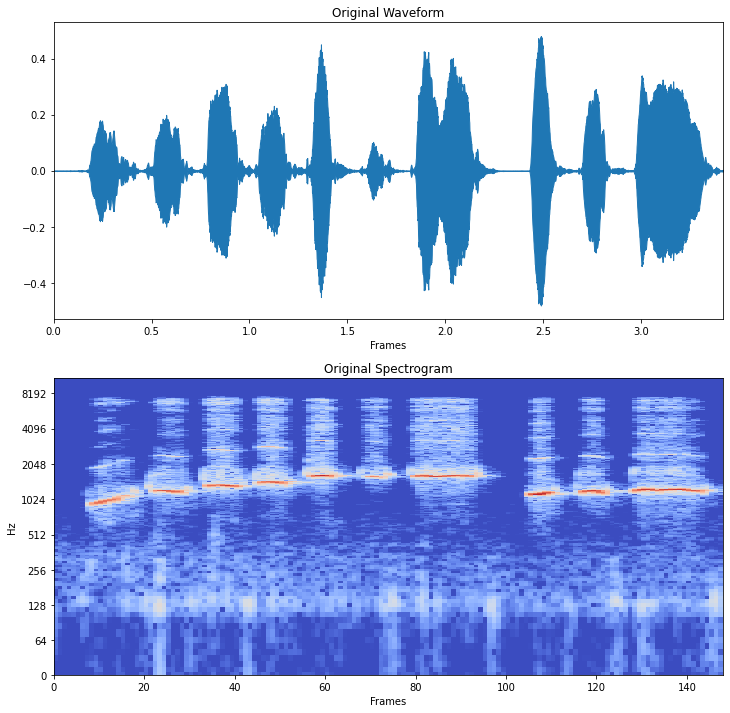
\includegraphics[width=0.5\textwidth]{dreamsound/original-waveform.png}
       \caption{Original Sound File: Whisteling}
       \label{fig:img-0}
\end{figure*}
YAMNet has been previously trained with 521 audio classes based on the AudioSet-YouTube \footnote{\url{https://research.google.com/audioset}} corpus. Since our prototype is meant for fast showcasing of the main DreamSound idea, this general raw audio database with short, mostly non-musical fragments. Therefore, we sacrificed any application of this system with other contextually/musically relevant sonic scenarios to favor a quick presentation of the idea. The second aspect relates to machine learning sonification. While most machine learning models have a way to visually represent data in graphs, there is very little research into the sonification of this data. Given that our prototipe uses sound as output, our approach is a sonification approach which takes advantage on listening to changes in the audio so as to grasp how a deep activation layer identifies sounds for classification. In fact, we have worked this prototype out with continuous sonic feedback throughout.

\begin{figure*}[htbp]
       \centering
              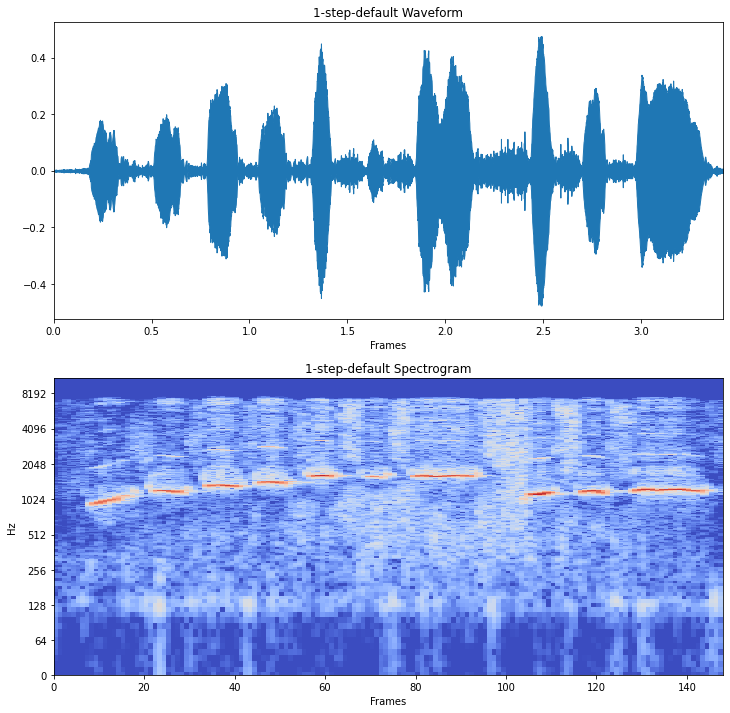
\includegraphics[width=0.5\textwidth]{dreamsound/1-step-default.png}
       \caption{One Step with default gradient addition}
       \label{fig:img-1}
\end{figure*}
\section{Method}
We based our method on the Deep Dream tutorial published by tensorflow, \footnote{\url{https://www.tensorflow.org/tutorials/generative/deepdream}} in which they implement Alexander Mordvintsev's original Deep Dream idea.\footnote{\url{https://ai.googleblog.com/2015/06/inceptionism-going-deeper-into-neural.html}} In general terms, the structure of the deep dream process involves inputting an image for classification,  grabbing the features obtained of one activation layer during that classification (aka. gradients), and combining the original image with the gradients in some way. In the tensorflow implementation, the gradients are added to the original image in small, gradual increments during a recursive process involving several passes. In our implementation, however, we had to introduce some modifications. Since we are dealing with audio, the 2-dimensional shapes of images had to be brought to one-dimensional sound arrays. Moreover, the combination of the original and the gradients is presented in different ways.
\begin{figure*}[htbp]
       \centering
              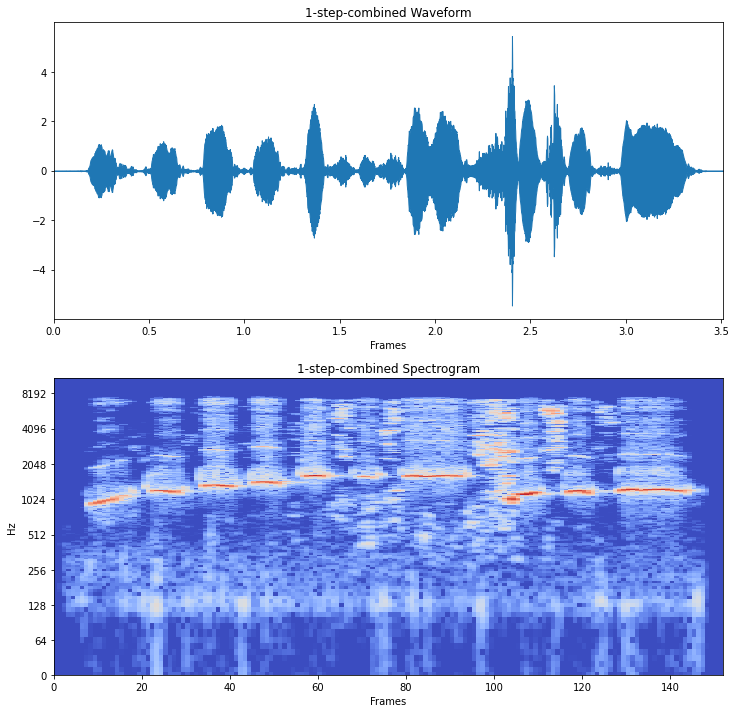
\includegraphics[width=0.5\textwidth]{dreamsound/1-step-combined.png}
       \caption{One step with original filtered with gradients}
       \label{fig:img-2}
\end{figure*}
\subsection{Algorithm Overview}
First, we pass a sound file through the model to obtain the activations with respect to one layer and get the loss across all audio frames. Then, we maximize the loss from these activations using gradient ascent with respect to the original sound file. Finally, we combine the gradients with the original sound to output a new, 'dreamed' sound.


\begin{figure*}[htbp]
       \centering
              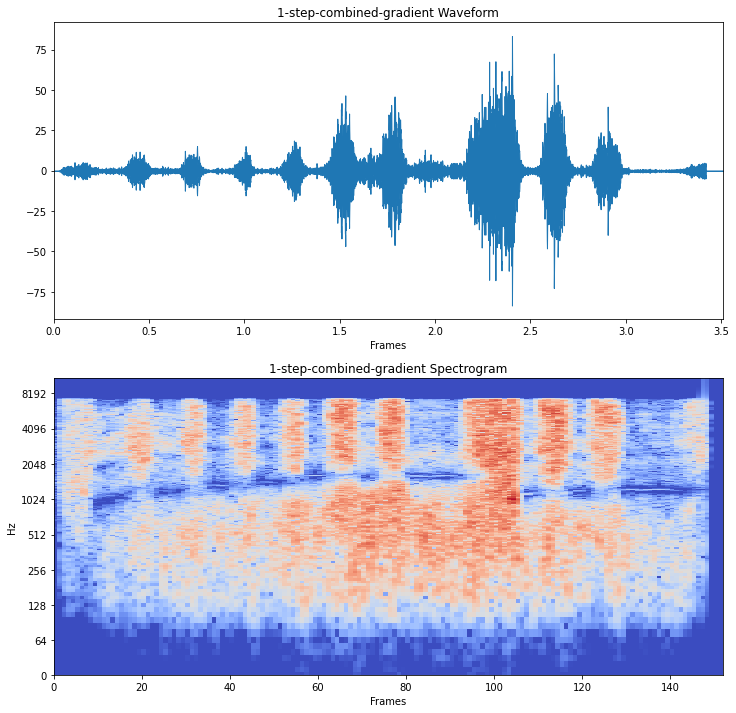
\includegraphics[width=0.5\textwidth]{dreamsound/1-step-combined-gradients.png}
       \caption{One step with gradients filtered with original}
       \label{fig:img-3}
\end{figure*}



\subsection{Calculate Loss}
We pass a sound file (See Figure \ref{fig:img-0}) through the model to obtain its activations (or scores) with respect to one layer (aka, the dream layer). Then, we take the mean accross all frames of the returned activations and return the maximum value which points to one specific class. In other words, we get the class that most represents the sound file so as to find the sum of all of its activations, thus representing the loss of the model with respect to the input.



\subsection{Gradient Ascent}
With the loss, we calcualte its gradient with respect to the input sound file, and maximize the loss so as to excite the features that most represent the input sound file within the network. In this sense, we are motivating the model to resurface what it's learnt. 


\subsection{Recursion}
Once we have the gradients, we can add them or combine them spectrally with the input sound file and listen to the output (See Figures \ref{fig:img-1}, \ref{fig:img-2} and \ref{fig:img-3}). However, if we iterate and recurse, we create a feedback loop that further excites the sonic output and we can define the number of steps and the step size of the recursion (See Figures \ref{fig:img-4}, \ref{fig:img-5}). In other words, we treat this as an feedback delay network effect with amount and amplitude values. Furthermore, we can take multiple layers simultaneously for the dream layers and see how affects the output (See Figures \ref{fig:img-6}, \ref{fig:img-7}).

\begin{figure*}[htbp]
       \centering
              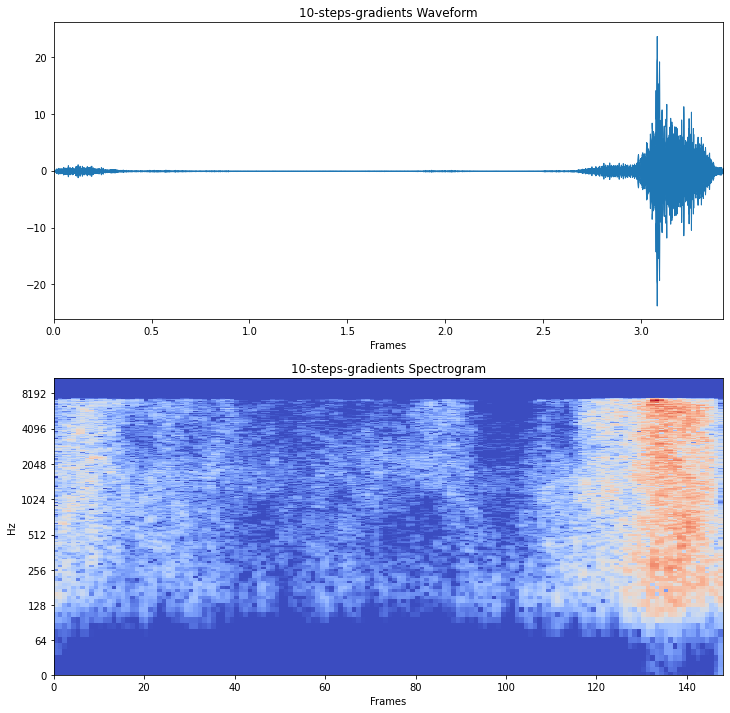
\includegraphics[width=0.5\textwidth]{dreamsound/10-steps-gradients.png}
       \caption{Recursively passing the gradients for 10 steps.}
       \label{fig:img-4}
\end{figure*}

\section{Results}
We have obtained several dreamed sound files with different parameter settings as can be seen on the presented figures across this paper.\footnote{The audio files can be listened to here: \url{https://github.com/fdch/dreamsound}} From these returned sounds, we can assess the validity of dreamsound as a deep dream implementation. In figures \ref{fig:img-1}, \ref{fig:img-2}, and \ref{fig:img-3}, we see the result of one step dream process, with different kinds of combinations between the gradients and the orignal sound. In the first example, we modify the sound usign the same method as in the deep dream tensorflow implementation. 

\begin{figure*}[htbp]
       \centering
              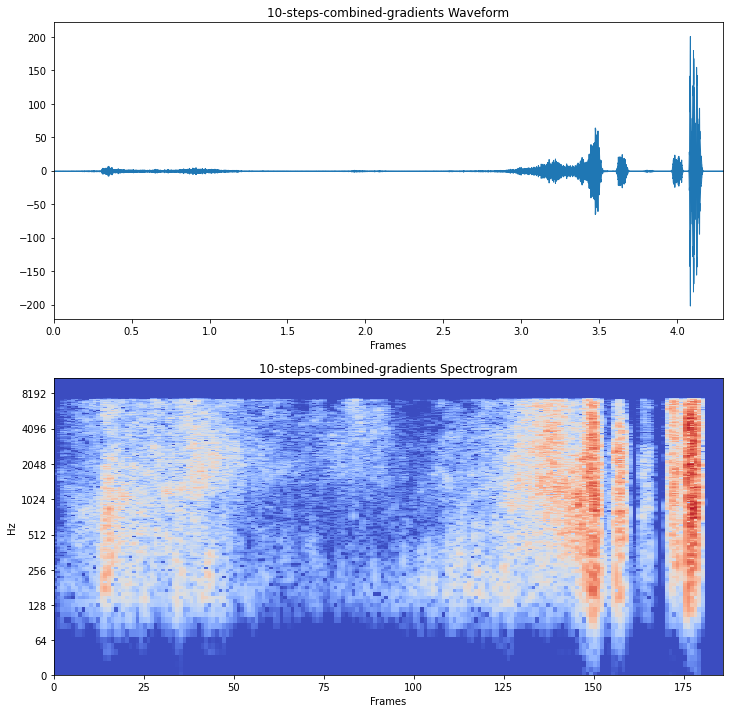
\includegraphics[width=0.5\textwidth]{dreamsound/10-steps-combined-gradients.png}
       \caption{Recursively passing the combined spectra of waveform and gradients (flipped) for 10 steps.}
       \label{fig:img-5}
\end{figure*}

This means that the gradients are added at some reduced value to the original sound file. From the result, we can listen to a slightly noisier signal. In comparison to the original sound, the noise within this new sound is enhanced when the original sound seems to fall back to silence, and it increments slightly in amplitude towards the middle section of the sound file's lenght. What we listen to here is the activations as they are represented sonically across all audio frames, so that louder portions represent the sections of the file where the most activations exists. This can be more accurately seen in Figure \ref{fig:img-3}, where we obtain the result of only sonifying the activations. However, in Figure \ref{fig:img-2}, we filter the original sound with the activations. This results in a much more insteresting sonic manipulation and result. The activations, since they evolve throghout the soundfile, create a dynamic filter concentrating towards the center of the file, which is when it resonates the most with the original sound file. This means that when we listen to the resonance, the network has the most accurate activations excited. For this step, we implemented a basic FFT filter withi tensorflow:

\begin{lstlisting}[language=Python][caption=A Custom FFT Filter in Tensorflow]
def filt(x,y,w=2048,h=128,m=0.01):
    # take sfft
    X = tf.signal.stft(x,w,h)
    Y = tf.signal.stft(y*m,w,h)
    # power spectrum of Y
    a = tf.math.abs(Y)**2
    # get rid of small values
    s = 0.5*(tf.math.sign(a-0.1)+1)
    a *= s 
    # apply filter
    r = a*tf.math.real(Y)
    i = a*tf.math.imag(Y)
    # convert to complex
    f = tf.dtypes.complex(r,i)
    # add together
    XY = X + f
    # compute the inverse
    out = tf.signal.inverse_stft(XY, w, h)
    
    return out
\end{lstlisting}
When applied recursively, this prototype projects its most promising results. In figures \ref{fig:img-4} and \ref{fig:img-5}, we can listen to the result of 10 iterations of the loss maximization loop acting on its own output. In the fist case, we feed only the gradients back to the loop, so we can see how these get washed out and clustered towards the end of the file. The sonic result reflects a drastic change with respect to the original, which has almost ---but not entirely so--- vanished. It is important to note that the frequency content of the gradient noise, at least aurally, corresponds to that of the original sound file. That is to say, both sounds, while dynamically different, can be catalogued into a related timbre. A more drastic result is in Figure \ref{fig:img-5}, where we feed back into the loop the gradients filtered with the sound file (i.e., a flipping these two), for 10 iterations. This results in a rhythmic variation of the original sound's rhythm. More closely, it sounds very much like Figure \ref{fig:img-3}, but washed and clustered towards the end of the file, as in Figure \ref{fig:img-5}. 

As a final test, we concatenated and summed multiple iterations performed on the last three layers of the network. This resulted in Figures  \ref{fig:img-6} and  \ref{fig:img-7}.

\begin{figure*}[htbp]
       \centering
              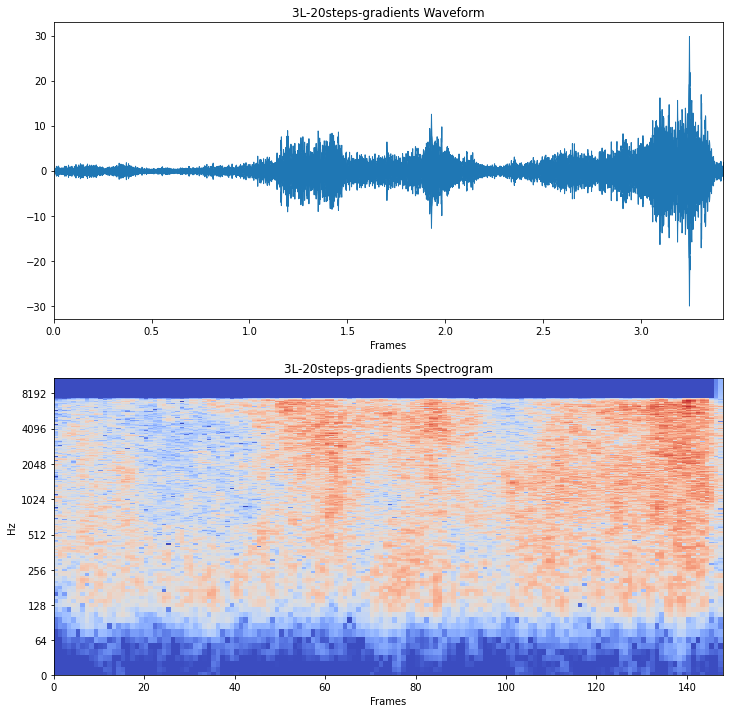
\includegraphics[width=0.5\textwidth]{dreamsound/3L-20steps-gradients.png}
       \caption{Taking last three layers, outputting gradients recursively for 20 steps.}
       \label{fig:img-6}
\end{figure*}
\begin{figure*}[htbp]
       \centering
              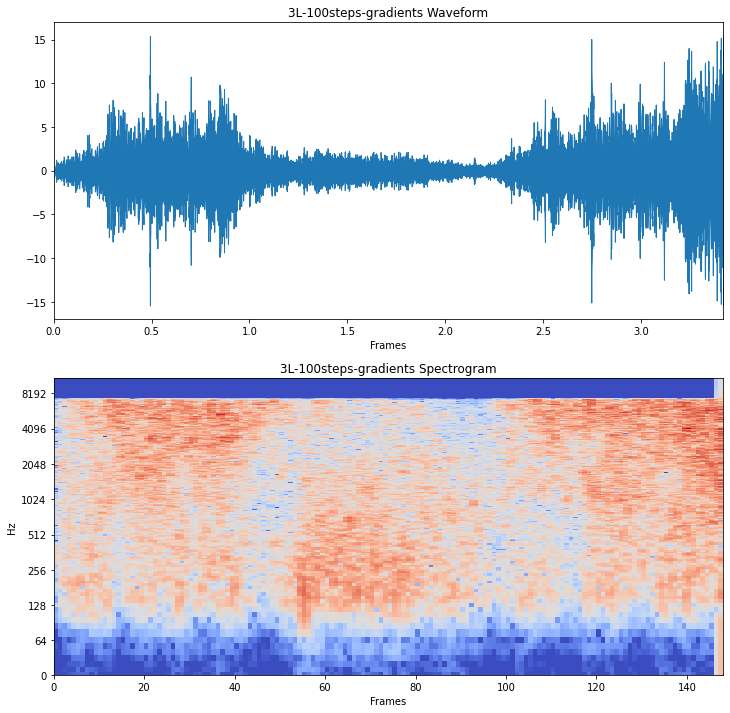
\includegraphics[width=0.5\textwidth]{dreamsound/L-100steps-gradients.png}
       \caption{Taking last 3 layers, for 100 steps, recursively feeding the gradients}
       \label{fig:img-7}
\end{figure*}
\section{Conclusions and Future Work}
We have presented a prototype adaptation of the Deep Dream project into an audio-based musical context using tensorflow and YAMNEt. We have contributed some research at the intersection of Deep Learning and audio-based musical tasks, and presented our results. The most interesting results occur when recursively applying an FFT filter built from the gradients obtained from an input soundfile and its loss. While our approach is tethered to a general sound database and a specific model, the techniques of gradient ascent for loss maximization of layer activations, and the FFT filter exposed in this paper are be portable enought for importing into other existing classification models for audio, such as for genre or musical instrument classification. Further, we plan on extending this project towards the creation of a database of dreamed sounds, with the capability to change models and other fft filtering techniques.

\section{Acknowledgments}
The authors would like to thank the reviewers, adding that the camera-ready paper will have a more detailed and verbose bibliographic section.
% -------------------------------------------------------------------------
% Either list references using the bibliography style file IEEEtran.bst
\bibliographystyle{IEEEtran}
\bibliography{dreamsound.bib}
%
% or list them by yourself
% \begin{thebibliography}{9}
% 
% \bibitem{icad2015web}
%   \url{http://www.icad.org}.
%
%\bibitem[1]{icad1} A.~Bee, C.D.~Player, and X.~Lastname, ``A correct citation,'' in {\it Proc. of the 1st Int. Conf. (IC)}, Helsinki, Finland, June 2001, pp. 1119-1134.  
%\bibitem[2]{icad2} E.~Zwicker and H.~Fastl, {\it Psychoacoustics: Facts and Models}, Springer-Verlag, Heidelberg, Germany, 1990.
%\bibitem[3]{icad3} M.R.~Smith, ``A good journal article,'' {\it J. Acoust. Soc. Am.}, vol. 110, no. 3, pp. 1598--1608, Mar. 2001.
% 
% \end{thebibliography}

\end{sloppy}
\end{document}
